%!TEX program = xelatex
\PassOptionsToPackage{dvipsnames,x11names,svgnames}{xcolor}
% \documentclass{beamer}                % Full presentation
\documentclass[trans]{beamer}       % Transparency mode (no overlays)
% \PassOptionsToPackage{gray}{xcolor} % Force grey colours for printing
% \documentclass[handout]{beamer}     % Handout mode


%% Graphics %%
\usepackage{fancybox,graphicx}
\usepackage{pgfpages}
\usepackage{tikz}
\usetikzlibrary{shapes,arrows,intersections,positioning,decorations.pathreplacing,calc}
\usepackage{pgfplots}
\pgfplotsset{compat=newest}


%% load custom sweave (listings) package %%
\usepackage{sweave}


%% Font features %%
\usepackage{lettrine}

\usepackage{unicode-math}
\usepackage{fontspec}
\usepackage{xeCJK} 
\usepackage{polyglossia}


\setmainlanguage{english}
\setotherlanguage{arabic}

\usefonttheme{professionalfonts} % use own font handling

% \setmainfont{Linux Libertine O}[Ligatures={Common,TeX}]
\setmainfont{Libertinus Serif}[Ligatures={Common,TeX}]
% \setsansfont{Linux Biolinum O}
\setsansfont{Libertinus Sans}
\setmonofont{Source Code Pro}[Ligatures={NoCommon},Scale=MatchLowercase,UprightFont={* Medium}]
\setmathfont{Libertinus Math}

\setCJKmainfont{標楷體} % for brush stroke on Windows 
\setCJKfamilyfont{korm}{Gungsuh}
\newfontfamily\arabicfont[Script=Arabic]{Amiri}
\newfontfamily\arabicfontsf[Script=Arabic]{Amiri}


\usepackage{metalogo}


%% Tables %%
\usepackage{booktabs}

%% Miscellaneous %%
\usepackage[os=win]{menukeys}

%%%%%%%%%%%%%%%%%%%%%%%%%%%%%%
% Custom functions
%%%%%%%%%%%%%%%%%%%%%%%%%%%%%%

% Custom colors
\definecolor{Cblue}{RGB}{59,102,178}
\definecolor{Cgreen}{RGB}{0,128,0}
\definecolor{Cred}{RGB}{184,0,0}

\newcommand{\highld}[1]{\textcolor<2->{Cblue}{#1}}
\newcommand{\highl}[1]{\textcolor{Cblue}{#1}}

\newcommand*\proitem{\item[\color{Cgreen}\resizebox{!}{1ex}{$\blacktriangleright$}]}
\newcommand*\conitem{\item[\color{Red}\resizebox{!}{1ex}{$\blacktriangleright$}]}

\newcommand{\qm}[1]{‘#1’}
\newcommand{\dqm}[1]{“#1”}
\newcommand{\gm}[1]{«#1»}

\newcommand{\ie}{\textit{i.\,e.},\xspace}
\newcommand{\eg}{\textit{e.\,g.},\xspace}

% define \authormail , 2-argument macro to get the author name and e-mail address 
% with hyperlink in the title page and footer, while separating text and pdf strings
\newcommand{\authormail}[2]{
  \author[\href{mailto:#2}{#1}]{\texorpdfstring{#1 \\ \href{mailto:#2}{\textsf{#2}}}{#1}}
}

\newenvironment{myquote}{\list{}{\leftmargin=0pt\rightmargin=10pt}\itshape\item[]}{\endlist}



\author{Matteo Sostero}
\authormail{Matteo Sostero}{m.sostero@sssup.it}
\institute{Sant'Anna School of Advanced Studies, Pisa}

\title{Title}
\subtitle{Subtitle}


\begin{document}


\begin{frame}
\includegraphics[scale=0.6]{SA_economics_logo_eng.pdf}
\maketitle
\end{frame}



\begin{frame}
\frametitle{Outline}
\tableofcontents
\end{frame}



\section{Blocks and lists}

\begin{frame}
\frametitle{Some lists and warnings}
\begin{itemize}[<+->]
\item First item
\item Second item
\item \alert{Important Warning!}
\item Hyperlink \highl{\hyperlink{Hayek-quote}{Hayek (1945)}} \only<4>{\hypertarget{Hayek-back}{}}
\end{itemize}
\pause[\thebeamerpauses]
\begin{alertblock}{Even more important warning!}
This is an important warning.
\end{alertblock}
\end{frame}


\begin{frame}
\frametitle{Why \LaTeX?}
\framesubtitle{From \url{http://www.ctan.org/what_is_tex.html}}
\begin{columns}[T]
\begin{column}{.46\textwidth}
\begin{block}{Output Quality}
\begin{itemize}
\item It has the best output.
\item It knows typesetting.
\end{itemize}
\end{block}
\uncover<3->{
  \begin{block}{Superior Engineering}
  \begin{itemize}
  \item It's fast.
  \item It's stable.
  \item It's not rigid (extensible).
  \item Plain text input.
  \item Many output types.
  \end{itemize}
  \end{block}
}
\end{column}

\begin{column}{.46\textwidth}
\uncover<2->{
  \begin{block}{Freedom}
  \begin{itemize}
  \item It's free.
  \item It runs anywhere.
  \end{itemize}
  \end{block}
}
\uncover<4->{
  \begin{block}{Popularity}
  \begin{itemize}
  \item It's the standard (in academia and science).
  \end{itemize}
  \end{block}
}
\end{column}
\end{columns}
\end{frame}



\section{Typesetting with \texorpdfstring{\XeLaTeX}{XeLaTeX}}

\begin{frame}%[fragile]
\frametitle{\XeLaTeX \ features}
  \begin{exampleblock}{Unicode support}
  \begin{columns}[T]
  \begin{column}{.45\textwidth}
  \renewcommand{\baselinestretch}{0.9}
  \begin{itemize}
  \item Arabic: \textarabic{العَرَبِيَّة}
  \item Armenian: {\fontspec{Times New Roman} հայերէն }
  \item Cyrillic: ру́сский
  \item Greek: ελληνικά
  \item Hebrew: עִבְרִית
  \end{itemize}
  \end{column}
  \begin{column}{.55\textwidth}
  \renewcommand{\baselinestretch}{0.9}
  \begin{itemize}
  \item Traditional Chinese: 繁體字
  \item Simplified Chinese: 简化字 
  \item Hiragana: {\CJKnospace ひらがな}
  \item Katakana: カタカナ
  \item Hangul: {\CJKfamily{korm} \CJKspace 한글}
  \end{itemize}
  \end{column}
  \end{columns}
\end{exampleblock}
\begin{exampleblock}{Advanced font features}
\renewcommand{\baselinestretch}{0.9}
\begin{itemize}
  \item Real small capitals: \textsc{AaBbWwXxYyZz}
  \item Old style numerals: \addfontfeatures{Numbers={OldStyle,Proportional}} 0123456789
  \item Common ligatures: ff fi fj fl ffi ffl ffj Th Qu
  \item Historical ligatures: \addfontfeatures{Ligatures={Rare,Historic}} Quest \& action. Just historic.
  \item Font-specific glyphs: \symbol{"E000} \symbol{"E009} \symbol{"E00A} \symbol{"E040} \symbol{"E001} \symbol{"E002} \symbol{"E003}
\end{itemize}
\end{exampleblock}
\end{frame}



\begin{frame}{Example blocks}
\begin{columns}[T]
\begin{column}{0.45\textwidth}
\begin{exampleblock}{Transparent uncover}
  \setbeamercovered{transparent}
  \begin{itemize}[<+->]
  \item Item 1
  \item Item 2
  \item Item 3
  \end{itemize}
\end{exampleblock}
\end{column}


\begin{column}{0.45\textwidth}
\begin{exampleblock}{Highlighting}
\begin{enumerate}[<alert@+>]
\setbeamercolor{alerted text}{fg=green!50!black}
\item Item 1
\item Item 2
\item Item 3
\end{enumerate}
\end{exampleblock}
\end{column}
\end{columns}
\end{frame}



\section{Code listings}

\begin{frame}[fragile]
\frametitle{Example of \R code}
Some code
\begin{Sinput}
binary <- function(i){
    a <- 2^(0:9); b <- a;
    lista <- list(NULL,NA,1,2,3,T,F)
    # Typeface for code is monospaced, comments are \LaTeX{}, slanted Roman (with math support: $\sqrt{x_{i}}$)
    function(x) sum(10^(0:9)[(x %% 2) != 0])
    print('a string')
}
\end{Sinput}

Some output of another \R{} command: \lil|print(...)|\\
\begin{Soutput}
 [1]  1  2  3  4  5  6  7  8  9 10
\end{Soutput}
% See http://texblog.org/2013/03/14/menukeys-typesetting-menu-sequences-directory-path-names-and-keyboard-shortcuts-in-latex/
For saving a file to the desktop, go to \menu[,]{File, Save As...} and navigate to \directory{Users/Username/Desktop}.\\
\medskip
Alternatively, use: \keys{\ctrl+\shift+S} and \keys{\ctrl+\return+\tab}.
\end{frame}



\section{Formulas}
\begin{frame}
\frametitle{Some impressive-looking formulas\ldots}
\begin{itemize}[<+->]
\item Meaningless expression:
\[
\frac{\partial \mathcal{L} \left(R(t), \phi\right)}{\partial t} \sim \left \lbrace \int_{-\infty}^{+\infty}
\frac{\widetilde{\mathcal{H}}(\gamma) \cdot \sqrt{\lim_{t\rightarrow\infty}\exp^{t-1}}}
     {\sum_{i=1}^\infty \mathbb{E}\left( \dot{x}_i^2\right)} \, \mathrm{d}t \right \rbrace^{-1}
\]
\item Matrices and greek letters
\[
\forall \Gamma \Delta\exists \Theta \otimes \mathbb{R} \succeq
\begin{bmatrix}
\alpha & \beta  & \gamma & \delta  & \varepsilon & \zeta & \eta   \\
\theta & \iota  & \kappa & \lambda & \mu         & \xi   & \pi    \\
\rho   & \sigma & \tau   & \phi    & \chi        & \psi  & \omega \\
\end{bmatrix}
=
\begin{bmatrix}
a_{\ell \kappa} & \ldots & \tau_{\ell i} \\
\vdots          & \ddots & \vdots        \\
\tau_{yj}       & \ldots & a_{nn}        \\
\end{bmatrix}
\]

\[
  \dot{a}\; \dot{x}\; \dot{y}\; \dot{w}\; \dot{z} \;\dot{\tau}
\]

% \[
% \dot{A}\; \dot{X}\; \dot{Y}\; \dot{W}\; \dot{Z} \;\dot{\Tau}
% \]
\end{itemize}
\end{frame}



\section{Plots}
\begin{frame}[fragile]
\frametitle{A plot}
\begin{center}
\begin{tikzpicture}
\begin{axis}[
  axis x line=middle,
  axis y line=left,
  domain=0:2,
  legend pos= north west,
  xlabel=$x$,
  ylabel=$ f(x)$,
  ytick={0,1,2,3},
  every axis y label/.style={at={(current axis.above origin)},anchor=north east}
]
\addplot[blue,mark=none,domain=0:2.01,samples=101] {(x^2)};
\addlegendentry{$x^2$}
\only<2>{
\addplot[red,mark=none,domain=0:2,samples=101] {sqrt(x)};
%\addplot[red,mark=none] gnuplot[domain=0:2,samples=101] {sqrt(x)};
\addlegendentry{$\sqrt{x}$}
}
\end{axis}
\end{tikzpicture}
\end{center}
\end{frame}


\begin{frame}[fragile]
\frametitle{A plot}
\begin{center}
\begin{tikzpicture}
\begin{axis}[
  height=5cm, width=10cm,
  xmin=-3.5, xmax=3.5,
  ymin=0, ymax=0.50,
  ytick={0},
  axis x line=bottom, axis y line=center,
  xlabel=$x$, ylabel=$f(x)$,
  every axis x label/.style={at={(current axis.right of origin)},anchor=north west},
  every axis y label/.style={at={(current axis.above origin)},anchor=north west}
]

% Draw normal curve
\addplot[Cblue,thick,smooth,domain=-3.5:3.5] {
  (1/(sqrt(2*pi)))*exp(-(x^2)/2) 
};

% Draw vertical line:
\only<2->{
  \draw [BrickRed,thick] (axis cs:-1.5,0) -- (axis cs:-1.5,0.1295176);
}

% Draw area
\only<3->{
  \addplot[fill=Cblue,opacity=0.4,smooth,domain=-3.225:-1.51] { (1/(sqrt(2*pi)))*exp(-(x^2)/2) } \closedcycle;
}
\end{axis}
\end{tikzpicture}

\end{center}
\end{frame}



\section{Tabulars}

\begin{frame}
\frametitle{Tables}
\begin{center}
\begin{tabular}{ccc}
\toprule
Title left &          & Title right \\
\midrule \pause
Left 1     & Center 1 & Right 1     \\
Left 2     & Center 2 & Right 2     \\
\bottomrule
\end{tabular}
\end{center}
\end{frame}



\section{References}

\begin{frame}
\frametitle{References}
\begin{thebibliography}{9}
\setbeamertemplate{bibliography item}[book]
\bibitem{1} Nelson, R. R., and Winter, S. G. 1982. \emph{An Evolutionary Theory of Economic Change.} Cambridge, Massachusetts: Belknap press.
\setbeamertemplate{bibliography item}[article]
\bibitem{2} Friedman, M. 1953. ``The Methodology of Positive Economics.'' In \emph{Essays in Positive Economics.} Chicago: University of Chicago Press.
\bibitem{3} Alchian, A. A. 1950. ``Uncertainty, Evolution and Economic Theory.'' \emph{Journal of Political Economy} 58: 211--222.
\setbeamertemplate{bibliography item}[book]
\bibitem{4} Koopmans, T. C. 1 957. \emph{Three Essays on the State of Economic Science.} New York: McGraw-Hill.
\end{thebibliography}
\end{frame}

\end{document}


\appendix

\begin{frame}[label=Hayek-quote]{Hayek's problem\hfilll \hyperlink{Hayek-back}{\beamerreturnbutton{Literature}}}
\begin{block}{}
\begin{columns}
\begin{column}{0.25\textwidth}
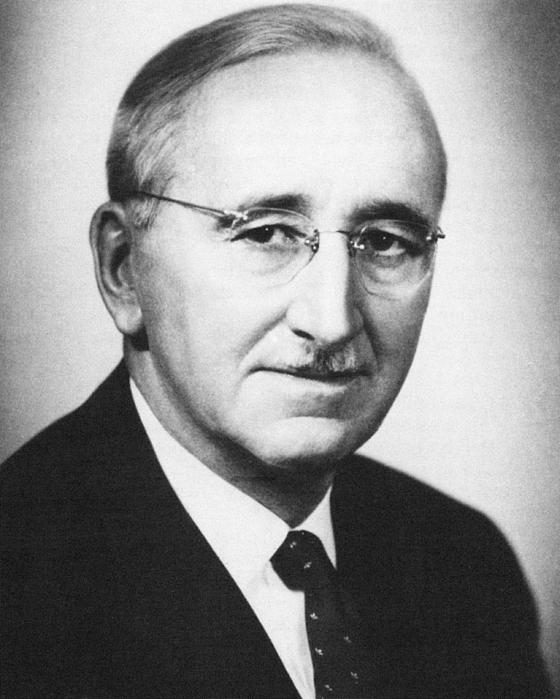
\includegraphics[width=\textwidth]{./Images/Hayek.jpg}
\end{column}
\begin{column}{0.7\textwidth}
\begin{quote}
\lettrine[findent=3.5pt,nindent=-3pt]{T}{he} peculiar character of the problem of a rational economic order is determined precisely by the fact that the knowledge of the circumstances of which we must make use never exists in concentrated or integrated form, but solely as the dispersed bits of incomplete and frequently contradictory knowledge which all the separate individuals possess.
\end{quote}
\end{column}
\end{columns}
%\flushright Hayek (1f945), \emph{The use of Knowledge in Society}\only<2>{, \highld{emphasis added}}
\end{block}
\end{frame}

\end{document}
